\documentclass[border=4pt]{standalone}
\usepackage{amsmath,amssymb,amsfonts}
\usepackage{xcolor,colortbl,array,booktabs,multirow}
\usepackage{tikz}
\usetikzlibrary{arrows, automata, backgrounds, calendar, chains, decorations,
    matrix, mindmap, patterns, petri, positioning, shadows, shapes.geometric,
    trees, shapes, decorations.pathreplacing, calc, tikzmark, arrows.meta}
\newcommand{\st}{\text{ s.t. }}
\newcommand{\x}{\mathbf{x}}
\renewcommand{\b}{\mathbf{b}}
\newcommand{\A}{\mathbf{A}}
\newcommand{\R}{\mathbb{R}}
\newcommand{\RR}{\mathbb{R}}
\newcommand{\Z}{\mathbb{Z}}
\newcommand{\ZZ}{\mathbb{Z}}
\begin{document}
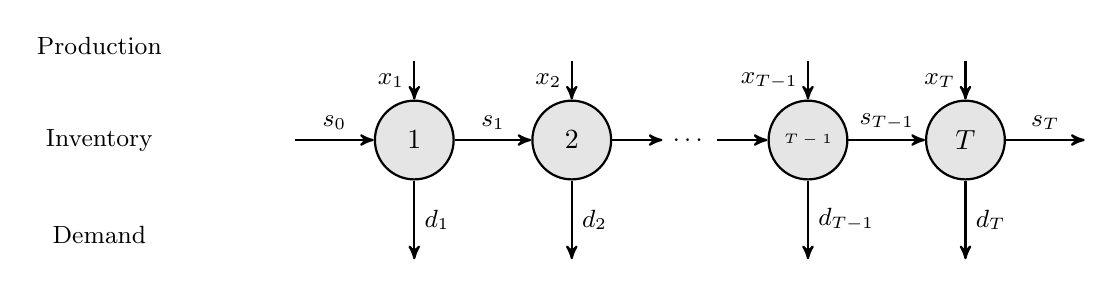
\begin{tikzpicture}[
    node distance=2cm, 
    thick, 
    >=stealth',
    every node/.style={font=\small},
    main/.style={circle, draw, fill=gray!20, minimum size=1cm, font=\normalsize}
]

% Nodes
\node[main] (1) {1};
\node[main, right of=1] (2) {2};
\node[right of=2, node distance=1.5cm] (dots) {\dots};
\node[main, right of=dots, node distance=1.5cm] (T1) {\tiny \(T-1\)};
\node[main, right of=T1] (T) {\(T\)};

% Arrows for Production
\foreach \i in {1,2,T}
    \draw[->] (\i) ++(0,1) -- node[left] {$x_\i$} (\i.north);
\foreach \i in {T1}
    \draw[->] (\i) ++(0,1) -- node[left] {$x_{T-1}$} (\i.north);
% Arrows for Inventory
\draw[<-] (1.west) -- ++(-1,0) node[midway, above] {$s_0$};
\draw[->] (1.east) -- node[midway, above] {$s_1$} (2.west);
\draw[->] (2.east) -- node[midway, above] {} (dots.west);
\draw[->] (dots.east) -- node[midway, above] {} (T1.west);
\draw[->] (T1.east) -- node[midway, above] {$s_{T-1}$} (T.west);
\draw[->] (T.east) -- ++(1,0) node[midway, above] {$s_T$};

% Arrows for Demand (using variables d_i)
\foreach \i in {1,2,T}
    \draw[->] (\i.south) -- ++(0,-1) node[midway, right] {$d_\i$};

\foreach \i in {T1}
    \draw[->] (\i.south) -- ++(0,-1) node[midway, right] {$d_{T-1}$};
% Labels
\node at (-4,1.2) {Production};
\node at (-4,0) {Inventory};
\node at (-4,-1.2) {Demand};

\end{tikzpicture}
\end{document}
